% Created by tikzDevice version 0.7.0 on 2014-07-26 02:55:47
% !TEX encoding = UTF-8 Unicode
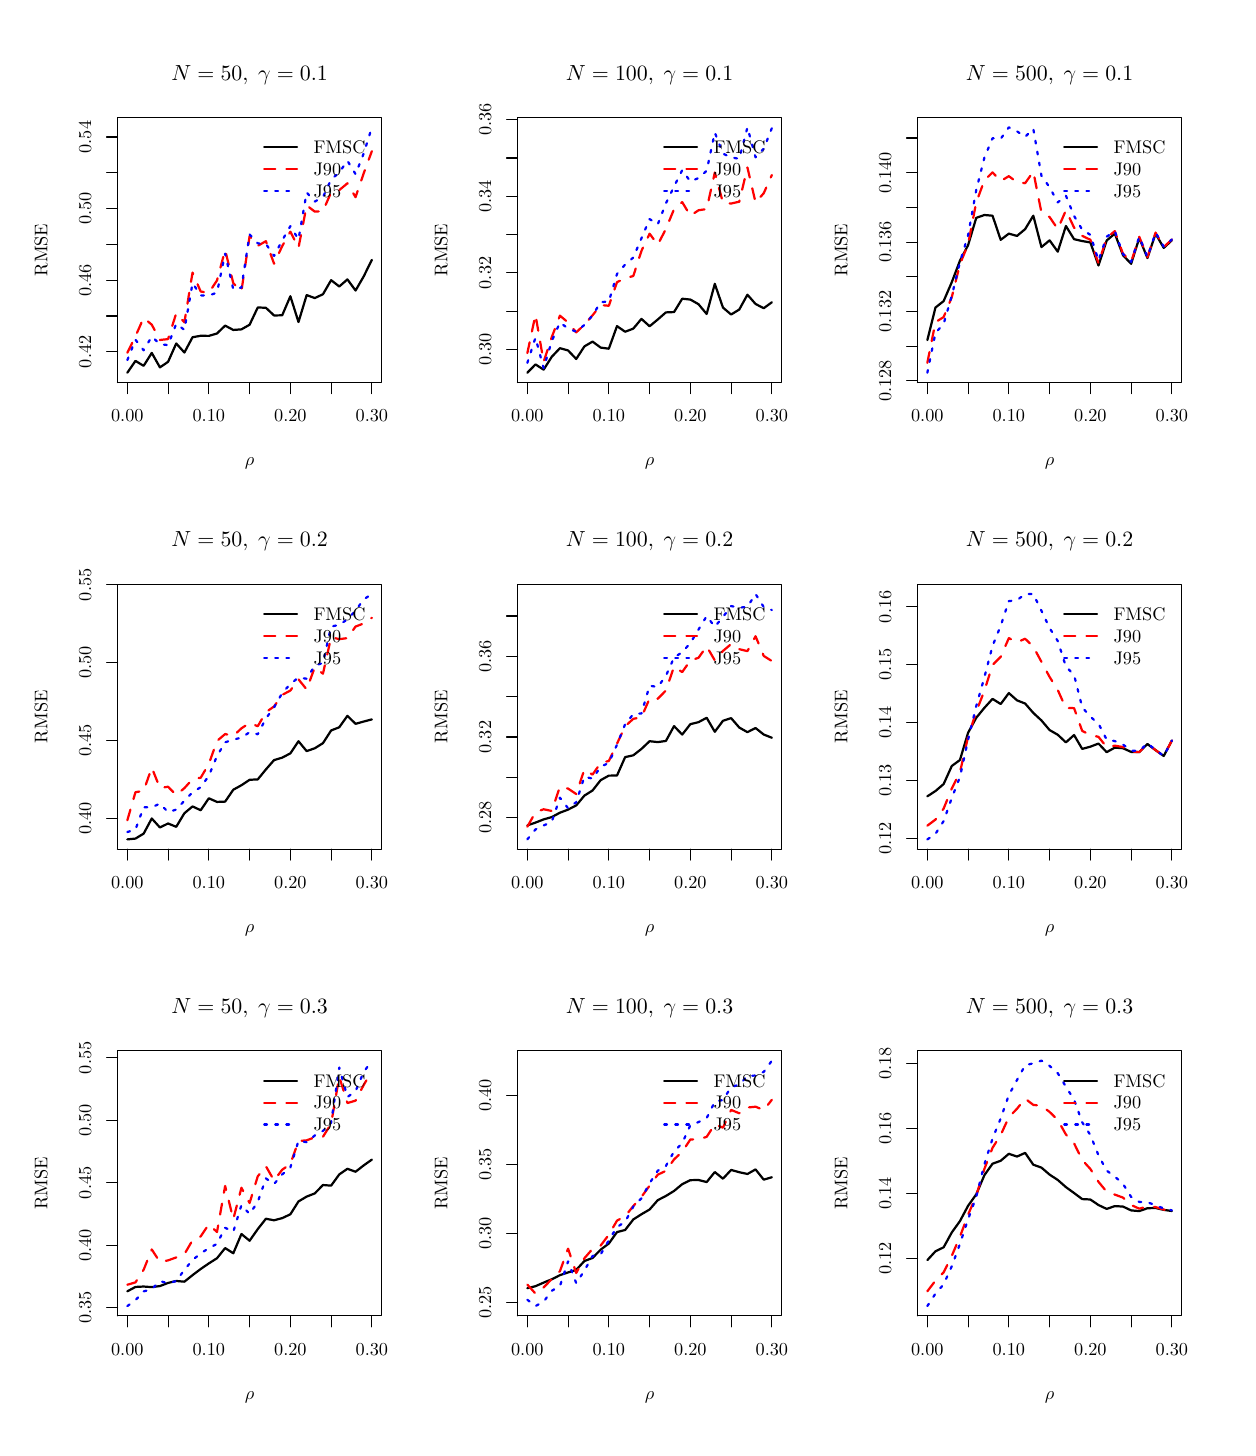
\begin{tikzpicture}[x=1pt,y=1pt]
\definecolor[named]{fillColor}{rgb}{1.00,1.00,1.00}
\path[use as bounding box,fill=fillColor,fill opacity=0.00] (0,0) rectangle (433.62,505.89);
\begin{scope}
\path[clip] ( 32.47,377.65) rectangle (127.91,473.42);
\definecolor[named]{drawColor}{rgb}{0.00,0.00,0.00}

\path[draw=drawColor,line width= 0.8pt,line join=round,line cap=round] ( 36.01,381.20) --
	( 38.95,385.47) --
	( 41.90,383.69) --
	( 44.84,388.36) --
	( 47.79,383.14) --
	( 50.73,385.13) --
	( 53.68,391.77) --
	( 56.63,388.50) --
	( 59.57,394.02) --
	( 62.52,394.55) --
	( 65.46,394.51) --
	( 68.41,395.38) --
	( 71.35,398.22) --
	( 74.30,396.66) --
	( 77.24,396.87) --
	( 80.19,398.54) --
	( 83.14,404.78) --
	( 86.08,404.67) --
	( 89.03,401.89) --
	( 91.97,401.95) --
	( 94.92,408.84) --
	( 97.86,399.52) --
	(100.81,409.25) --
	(103.75,408.18) --
	(106.70,409.56) --
	(109.65,414.65) --
	(112.59,412.36) --
	(115.54,414.92) --
	(118.48,410.90) --
	(121.43,416.02) --
	(124.37,422.00);
\end{scope}
\begin{scope}
\path[clip] (  0.00,  0.00) rectangle (433.62,505.89);
\definecolor[named]{drawColor}{rgb}{0.00,0.00,0.00}

\path[draw=drawColor,line width= 0.4pt,line join=round,line cap=round] ( 36.01,377.65) -- (124.37,377.65);

\path[draw=drawColor,line width= 0.4pt,line join=round,line cap=round] ( 36.01,377.65) -- ( 36.01,373.69);

\path[draw=drawColor,line width= 0.4pt,line join=round,line cap=round] ( 50.73,377.65) -- ( 50.73,373.69);

\path[draw=drawColor,line width= 0.4pt,line join=round,line cap=round] ( 65.46,377.65) -- ( 65.46,373.69);

\path[draw=drawColor,line width= 0.4pt,line join=round,line cap=round] ( 80.19,377.65) -- ( 80.19,373.69);

\path[draw=drawColor,line width= 0.4pt,line join=round,line cap=round] ( 94.92,377.65) -- ( 94.92,373.69);

\path[draw=drawColor,line width= 0.4pt,line join=round,line cap=round] (109.65,377.65) -- (109.65,373.69);

\path[draw=drawColor,line width= 0.4pt,line join=round,line cap=round] (124.37,377.65) -- (124.37,373.69);

\node[text=drawColor,anchor=base,inner sep=0pt, outer sep=0pt, scale=  0.66] at ( 36.01,363.40) {0.00};

\node[text=drawColor,anchor=base,inner sep=0pt, outer sep=0pt, scale=  0.66] at ( 65.46,363.40) {0.10};

\node[text=drawColor,anchor=base,inner sep=0pt, outer sep=0pt, scale=  0.66] at ( 94.92,363.40) {0.20};

\node[text=drawColor,anchor=base,inner sep=0pt, outer sep=0pt, scale=  0.66] at (124.37,363.40) {0.30};

\path[draw=drawColor,line width= 0.4pt,line join=round,line cap=round] ( 32.47,388.75) -- ( 32.47,466.36);

\path[draw=drawColor,line width= 0.4pt,line join=round,line cap=round] ( 32.47,388.75) -- ( 28.51,388.75);

\path[draw=drawColor,line width= 0.4pt,line join=round,line cap=round] ( 32.47,401.68) -- ( 28.51,401.68);

\path[draw=drawColor,line width= 0.4pt,line join=round,line cap=round] ( 32.47,414.62) -- ( 28.51,414.62);

\path[draw=drawColor,line width= 0.4pt,line join=round,line cap=round] ( 32.47,427.55) -- ( 28.51,427.55);

\path[draw=drawColor,line width= 0.4pt,line join=round,line cap=round] ( 32.47,440.49) -- ( 28.51,440.49);

\path[draw=drawColor,line width= 0.4pt,line join=round,line cap=round] ( 32.47,453.42) -- ( 28.51,453.42);

\path[draw=drawColor,line width= 0.4pt,line join=round,line cap=round] ( 32.47,466.36) -- ( 28.51,466.36);

\node[text=drawColor,rotate= 90.00,anchor=base,inner sep=0pt, outer sep=0pt, scale=  0.66] at ( 22.97,388.75) {0.42};

\node[text=drawColor,rotate= 90.00,anchor=base,inner sep=0pt, outer sep=0pt, scale=  0.66] at ( 22.97,414.62) {0.46};

\node[text=drawColor,rotate= 90.00,anchor=base,inner sep=0pt, outer sep=0pt, scale=  0.66] at ( 22.97,440.49) {0.50};

\node[text=drawColor,rotate= 90.00,anchor=base,inner sep=0pt, outer sep=0pt, scale=  0.66] at ( 22.97,466.36) {0.54};

\path[draw=drawColor,line width= 0.4pt,line join=round,line cap=round] ( 32.47,377.65) --
	(127.91,377.65) --
	(127.91,473.42) --
	( 32.47,473.42) --
	( 32.47,377.65);
\end{scope}
\begin{scope}
\path[clip] (  0.00,337.26) rectangle (144.54,505.89);
\definecolor[named]{drawColor}{rgb}{0.00,0.00,0.00}

\node[text=drawColor,anchor=base,inner sep=0pt, outer sep=0pt, scale=  0.79] at ( 80.19,486.92) {\bfseries $N=50, \;\gamma=0.1$};

\node[text=drawColor,anchor=base,inner sep=0pt, outer sep=0pt, scale=  0.66] at ( 80.19,347.56) {$\rho$};

\node[text=drawColor,rotate= 90.00,anchor=base,inner sep=0pt, outer sep=0pt, scale=  0.66] at (  7.13,425.53) {RMSE};
\end{scope}
\begin{scope}
\path[clip] ( 32.47,377.65) rectangle (127.91,473.42);
\definecolor[named]{drawColor}{rgb}{1.00,0.00,0.00}

\path[draw=drawColor,line width= 0.8pt,dash pattern=on 4pt off 4pt ,line join=round,line cap=round] ( 36.01,388.42) --
	( 38.95,394.36) --
	( 41.90,401.04) --
	( 44.84,398.56) --
	( 47.79,393.04) --
	( 50.73,393.35) --
	( 53.68,402.67) --
	( 56.63,399.40) --
	( 59.57,417.39) --
	( 62.52,410.55) --
	( 65.46,410.07) --
	( 68.41,414.55) --
	( 71.35,425.55) --
	( 74.30,413.56) --
	( 77.24,410.68) --
	( 80.19,430.57) --
	( 83.14,427.05) --
	( 86.08,428.74) --
	( 89.03,420.60) --
	( 91.97,426.95) --
	( 94.92,432.18) --
	( 97.86,426.35) --
	(100.81,441.64) --
	(103.75,439.42) --
	(106.70,439.60) --
	(109.65,446.39) --
	(112.59,447.19) --
	(115.54,449.65) --
	(118.48,444.63) --
	(121.43,453.29) --
	(124.37,461.25);
\definecolor[named]{drawColor}{rgb}{0.00,0.00,1.00}

\path[draw=drawColor,line width= 0.8pt,dash pattern=on 1pt off 3pt ,line join=round,line cap=round] ( 36.01,385.77) --
	( 38.95,393.12) --
	( 41.90,389.32) --
	( 44.84,394.27) --
	( 47.79,391.50) --
	( 50.73,391.19) --
	( 53.68,398.88) --
	( 56.63,396.68) --
	( 59.57,413.56) --
	( 62.52,409.15) --
	( 65.46,409.08) --
	( 68.41,410.16) --
	( 71.35,424.23) --
	( 74.30,411.31) --
	( 77.24,411.97) --
	( 80.19,431.17) --
	( 83.14,427.95) --
	( 86.08,427.78) --
	( 89.03,423.41) --
	( 91.97,429.01) --
	( 94.92,434.17) --
	( 97.86,429.39) --
	(100.81,446.33) --
	(103.75,443.05) --
	(106.70,444.68) --
	(109.65,451.01) --
	(112.59,453.57) --
	(115.54,457.79) --
	(118.48,452.96) --
	(121.43,460.46) --
	(124.37,469.87);
\definecolor[named]{drawColor}{rgb}{0.00,0.00,0.00}

\path[draw=drawColor,line width= 0.8pt,line join=round,line cap=round] ( 85.47,462.63) -- ( 97.35,462.63);
\definecolor[named]{drawColor}{rgb}{1.00,0.00,0.00}

\path[draw=drawColor,line width= 0.8pt,dash pattern=on 4pt off 4pt ,line join=round,line cap=round] ( 85.47,454.71) -- ( 97.35,454.71);
\definecolor[named]{drawColor}{rgb}{0.00,0.00,1.00}

\path[draw=drawColor,line width= 0.8pt,dash pattern=on 1pt off 3pt ,line join=round,line cap=round] ( 85.47,446.79) -- ( 97.35,446.79);
\definecolor[named]{drawColor}{rgb}{0.00,0.00,0.00}

\node[text=drawColor,anchor=base west,inner sep=0pt, outer sep=0pt, scale=  0.66] at (103.29,460.35) {FMSC};

\node[text=drawColor,anchor=base west,inner sep=0pt, outer sep=0pt, scale=  0.66] at (103.29,452.43) {J90};

\node[text=drawColor,anchor=base west,inner sep=0pt, outer sep=0pt, scale=  0.66] at (103.29,444.51) {J95};
\end{scope}
\begin{scope}
\path[clip] (177.01,377.65) rectangle (272.45,473.42);
\definecolor[named]{drawColor}{rgb}{0.00,0.00,0.00}

\path[draw=drawColor,line width= 0.8pt,line join=round,line cap=round] (180.55,381.20) --
	(183.49,384.20) --
	(186.44,382.31) --
	(189.38,386.96) --
	(192.33,390.07) --
	(195.27,389.25) --
	(198.22,386.17) --
	(201.17,390.71) --
	(204.11,392.45) --
	(207.06,390.28) --
	(210.00,389.88) --
	(212.95,398.04) --
	(215.89,396.01) --
	(218.84,397.14) --
	(221.78,400.66) --
	(224.73,397.99) --
	(227.68,400.43) --
	(230.62,403.00) --
	(233.57,403.12) --
	(236.51,407.94) --
	(239.46,407.64) --
	(242.40,405.96) --
	(245.35,402.43) --
	(248.29,413.32) --
	(251.24,404.74) --
	(254.19,402.23) --
	(257.13,404.04) --
	(260.08,409.39) --
	(263.02,406.04) --
	(265.97,404.51) --
	(268.91,406.66);
\end{scope}
\begin{scope}
\path[clip] (  0.00,  0.00) rectangle (433.62,505.89);
\definecolor[named]{drawColor}{rgb}{0.00,0.00,0.00}

\path[draw=drawColor,line width= 0.4pt,line join=round,line cap=round] (180.55,377.65) -- (268.91,377.65);

\path[draw=drawColor,line width= 0.4pt,line join=round,line cap=round] (180.55,377.65) -- (180.55,373.69);

\path[draw=drawColor,line width= 0.4pt,line join=round,line cap=round] (195.27,377.65) -- (195.27,373.69);

\path[draw=drawColor,line width= 0.4pt,line join=round,line cap=round] (210.00,377.65) -- (210.00,373.69);

\path[draw=drawColor,line width= 0.4pt,line join=round,line cap=round] (224.73,377.65) -- (224.73,373.69);

\path[draw=drawColor,line width= 0.4pt,line join=round,line cap=round] (239.46,377.65) -- (239.46,373.69);

\path[draw=drawColor,line width= 0.4pt,line join=round,line cap=round] (254.19,377.65) -- (254.19,373.69);

\path[draw=drawColor,line width= 0.4pt,line join=round,line cap=round] (268.91,377.65) -- (268.91,373.69);

\node[text=drawColor,anchor=base,inner sep=0pt, outer sep=0pt, scale=  0.66] at (180.55,363.40) {0.00};

\node[text=drawColor,anchor=base,inner sep=0pt, outer sep=0pt, scale=  0.66] at (210.00,363.40) {0.10};

\node[text=drawColor,anchor=base,inner sep=0pt, outer sep=0pt, scale=  0.66] at (239.46,363.40) {0.20};

\node[text=drawColor,anchor=base,inner sep=0pt, outer sep=0pt, scale=  0.66] at (268.91,363.40) {0.30};

\path[draw=drawColor,line width= 0.4pt,line join=round,line cap=round] (177.01,389.58) -- (177.01,472.64);

\path[draw=drawColor,line width= 0.4pt,line join=round,line cap=round] (177.01,389.58) -- (173.05,389.58);

\path[draw=drawColor,line width= 0.4pt,line join=round,line cap=round] (177.01,403.42) -- (173.05,403.42);

\path[draw=drawColor,line width= 0.4pt,line join=round,line cap=round] (177.01,417.27) -- (173.05,417.27);

\path[draw=drawColor,line width= 0.4pt,line join=round,line cap=round] (177.01,431.11) -- (173.05,431.11);

\path[draw=drawColor,line width= 0.4pt,line join=round,line cap=round] (177.01,444.95) -- (173.05,444.95);

\path[draw=drawColor,line width= 0.4pt,line join=round,line cap=round] (177.01,458.80) -- (173.05,458.80);

\path[draw=drawColor,line width= 0.4pt,line join=round,line cap=round] (177.01,472.64) -- (173.05,472.64);

\node[text=drawColor,rotate= 90.00,anchor=base,inner sep=0pt, outer sep=0pt, scale=  0.66] at (167.51,389.58) {0.30};

\node[text=drawColor,rotate= 90.00,anchor=base,inner sep=0pt, outer sep=0pt, scale=  0.66] at (167.51,417.27) {0.32};

\node[text=drawColor,rotate= 90.00,anchor=base,inner sep=0pt, outer sep=0pt, scale=  0.66] at (167.51,444.95) {0.34};

\node[text=drawColor,rotate= 90.00,anchor=base,inner sep=0pt, outer sep=0pt, scale=  0.66] at (167.51,472.64) {0.36};

\path[draw=drawColor,line width= 0.4pt,line join=round,line cap=round] (177.01,377.65) --
	(272.45,377.65) --
	(272.45,473.42) --
	(177.01,473.42) --
	(177.01,377.65);
\end{scope}
\begin{scope}
\path[clip] (144.54,337.26) rectangle (289.08,505.89);
\definecolor[named]{drawColor}{rgb}{0.00,0.00,0.00}

\node[text=drawColor,anchor=base,inner sep=0pt, outer sep=0pt, scale=  0.79] at (224.73,486.92) {\bfseries $N=100, \;\gamma=0.1$};

\node[text=drawColor,anchor=base,inner sep=0pt, outer sep=0pt, scale=  0.66] at (224.73,347.56) {$\rho$};

\node[text=drawColor,rotate= 90.00,anchor=base,inner sep=0pt, outer sep=0pt, scale=  0.66] at (151.67,425.53) {RMSE};
\end{scope}
\begin{scope}
\path[clip] (177.01,377.65) rectangle (272.45,473.42);
\definecolor[named]{drawColor}{rgb}{1.00,0.00,0.00}

\path[draw=drawColor,line width= 0.8pt,dash pattern=on 4pt off 4pt ,line join=round,line cap=round] (180.55,388.28) --
	(183.49,402.14) --
	(186.44,385.14) --
	(189.38,394.06) --
	(192.33,401.83) --
	(195.27,399.35) --
	(198.22,395.78) --
	(201.17,398.58) --
	(204.11,401.95) --
	(207.06,405.64) --
	(210.00,405.40) --
	(212.95,413.91) --
	(215.89,415.35) --
	(218.84,416.15) --
	(221.78,425.21) --
	(224.73,431.43) --
	(227.68,427.48) --
	(230.62,433.15) --
	(233.57,440.32) --
	(236.51,442.85) --
	(239.46,437.93) --
	(242.40,439.91) --
	(245.35,440.34) --
	(248.29,453.53) --
	(251.24,442.63) --
	(254.19,442.34) --
	(257.13,443.00) --
	(260.08,455.37) --
	(263.02,442.69) --
	(265.97,446.07) --
	(268.91,452.65);
\definecolor[named]{drawColor}{rgb}{0.00,0.00,1.00}

\path[draw=drawColor,line width= 0.8pt,dash pattern=on 1pt off 3pt ,line join=round,line cap=round] (180.55,384.76) --
	(183.49,393.86) --
	(186.44,382.84) --
	(189.38,392.64) --
	(192.33,399.34) --
	(195.27,397.19) --
	(198.22,396.04) --
	(201.17,398.48) --
	(204.11,401.91) --
	(207.06,406.72) --
	(210.00,406.91) --
	(212.95,416.88) --
	(215.89,420.28) --
	(218.84,422.83) --
	(221.78,429.77) --
	(224.73,436.72) --
	(227.68,434.82) --
	(230.62,442.38) --
	(233.57,448.48) --
	(236.51,454.37) --
	(239.46,450.32) --
	(242.40,451.54) --
	(245.35,454.18) --
	(248.29,468.00) --
	(251.24,460.37) --
	(254.19,459.00) --
	(257.13,458.50) --
	(260.08,469.87) --
	(263.02,459.05) --
	(265.97,462.14) --
	(268.91,469.60);
\definecolor[named]{drawColor}{rgb}{0.00,0.00,0.00}

\path[draw=drawColor,line width= 0.8pt,line join=round,line cap=round] (230.01,462.63) -- (241.89,462.63);
\definecolor[named]{drawColor}{rgb}{1.00,0.00,0.00}

\path[draw=drawColor,line width= 0.8pt,dash pattern=on 4pt off 4pt ,line join=round,line cap=round] (230.01,454.71) -- (241.89,454.71);
\definecolor[named]{drawColor}{rgb}{0.00,0.00,1.00}

\path[draw=drawColor,line width= 0.8pt,dash pattern=on 1pt off 3pt ,line join=round,line cap=round] (230.01,446.79) -- (241.89,446.79);
\definecolor[named]{drawColor}{rgb}{0.00,0.00,0.00}

\node[text=drawColor,anchor=base west,inner sep=0pt, outer sep=0pt, scale=  0.66] at (247.83,460.35) {FMSC};

\node[text=drawColor,anchor=base west,inner sep=0pt, outer sep=0pt, scale=  0.66] at (247.83,452.43) {J90};

\node[text=drawColor,anchor=base west,inner sep=0pt, outer sep=0pt, scale=  0.66] at (247.83,444.51) {J95};
\end{scope}
\begin{scope}
\path[clip] (321.55,377.65) rectangle (416.99,473.42);
\definecolor[named]{drawColor}{rgb}{0.00,0.00,0.00}

\path[draw=drawColor,line width= 0.8pt,line join=round,line cap=round] (325.09,392.99) --
	(328.03,404.76) --
	(330.98,407.09) --
	(333.92,413.91) --
	(336.87,421.67) --
	(339.81,427.28) --
	(342.76,437.16) --
	(345.71,438.19) --
	(348.65,437.94) --
	(351.60,429.22) --
	(354.54,431.46) --
	(357.49,430.63) --
	(360.43,433.09) --
	(363.38,437.96) --
	(366.32,426.60) --
	(369.27,429.03) --
	(372.22,424.94) --
	(375.16,434.22) --
	(378.11,429.46) --
	(381.05,428.78) --
	(384.00,428.28) --
	(386.94,419.95) --
	(389.89,428.96) --
	(392.83,431.48) --
	(395.78,423.66) --
	(398.73,420.56) --
	(401.67,429.90) --
	(404.62,422.63) --
	(407.56,431.44) --
	(410.51,426.30) --
	(413.45,429.04);
\end{scope}
\begin{scope}
\path[clip] (  0.00,  0.00) rectangle (433.62,505.89);
\definecolor[named]{drawColor}{rgb}{0.00,0.00,0.00}

\path[draw=drawColor,line width= 0.4pt,line join=round,line cap=round] (325.09,377.65) -- (413.45,377.65);

\path[draw=drawColor,line width= 0.4pt,line join=round,line cap=round] (325.09,377.65) -- (325.09,373.69);

\path[draw=drawColor,line width= 0.4pt,line join=round,line cap=round] (339.81,377.65) -- (339.81,373.69);

\path[draw=drawColor,line width= 0.4pt,line join=round,line cap=round] (354.54,377.65) -- (354.54,373.69);

\path[draw=drawColor,line width= 0.4pt,line join=round,line cap=round] (369.27,377.65) -- (369.27,373.69);

\path[draw=drawColor,line width= 0.4pt,line join=round,line cap=round] (384.00,377.65) -- (384.00,373.69);

\path[draw=drawColor,line width= 0.4pt,line join=round,line cap=round] (398.73,377.65) -- (398.73,373.69);

\path[draw=drawColor,line width= 0.4pt,line join=round,line cap=round] (413.45,377.65) -- (413.45,373.69);

\node[text=drawColor,anchor=base,inner sep=0pt, outer sep=0pt, scale=  0.66] at (325.09,363.40) {0.00};

\node[text=drawColor,anchor=base,inner sep=0pt, outer sep=0pt, scale=  0.66] at (354.54,363.40) {0.10};

\node[text=drawColor,anchor=base,inner sep=0pt, outer sep=0pt, scale=  0.66] at (384.00,363.40) {0.20};

\node[text=drawColor,anchor=base,inner sep=0pt, outer sep=0pt, scale=  0.66] at (413.45,363.40) {0.30};

\path[draw=drawColor,line width= 0.4pt,line join=round,line cap=round] (321.55,378.28) -- (321.55,466.01);

\path[draw=drawColor,line width= 0.4pt,line join=round,line cap=round] (321.55,378.28) -- (317.59,378.28);

\path[draw=drawColor,line width= 0.4pt,line join=round,line cap=round] (321.55,390.81) -- (317.59,390.81);

\path[draw=drawColor,line width= 0.4pt,line join=round,line cap=round] (321.55,403.34) -- (317.59,403.34);

\path[draw=drawColor,line width= 0.4pt,line join=round,line cap=round] (321.55,415.88) -- (317.59,415.88);

\path[draw=drawColor,line width= 0.4pt,line join=round,line cap=round] (321.55,428.41) -- (317.59,428.41);

\path[draw=drawColor,line width= 0.4pt,line join=round,line cap=round] (321.55,440.95) -- (317.59,440.95);

\path[draw=drawColor,line width= 0.4pt,line join=round,line cap=round] (321.55,453.48) -- (317.59,453.48);

\path[draw=drawColor,line width= 0.4pt,line join=round,line cap=round] (321.55,466.01) -- (317.59,466.01);

\node[text=drawColor,rotate= 90.00,anchor=base,inner sep=0pt, outer sep=0pt, scale=  0.66] at (312.05,378.28) {0.128};

\node[text=drawColor,rotate= 90.00,anchor=base,inner sep=0pt, outer sep=0pt, scale=  0.66] at (312.05,403.34) {0.132};

\node[text=drawColor,rotate= 90.00,anchor=base,inner sep=0pt, outer sep=0pt, scale=  0.66] at (312.05,428.41) {0.136};

\node[text=drawColor,rotate= 90.00,anchor=base,inner sep=0pt, outer sep=0pt, scale=  0.66] at (312.05,453.48) {0.140};

\path[draw=drawColor,line width= 0.4pt,line join=round,line cap=round] (321.55,377.65) --
	(416.99,377.65) --
	(416.99,473.42) --
	(321.55,473.42) --
	(321.55,377.65);
\end{scope}
\begin{scope}
\path[clip] (289.08,337.26) rectangle (433.62,505.89);
\definecolor[named]{drawColor}{rgb}{0.00,0.00,0.00}

\node[text=drawColor,anchor=base,inner sep=0pt, outer sep=0pt, scale=  0.79] at (369.27,486.92) {\bfseries $N=500, \;\gamma=0.1$};

\node[text=drawColor,anchor=base,inner sep=0pt, outer sep=0pt, scale=  0.66] at (369.27,347.56) {$\rho$};

\node[text=drawColor,rotate= 90.00,anchor=base,inner sep=0pt, outer sep=0pt, scale=  0.66] at (296.21,425.54) {RMSE};
\end{scope}
\begin{scope}
\path[clip] (321.55,377.65) rectangle (416.99,473.42);
\definecolor[named]{drawColor}{rgb}{1.00,0.00,0.00}

\path[draw=drawColor,line width= 0.8pt,dash pattern=on 4pt off 4pt ,line join=round,line cap=round] (325.09,384.76) --
	(328.03,399.47) --
	(330.98,401.31) --
	(333.92,408.49) --
	(336.87,420.40) --
	(339.81,427.59) --
	(342.76,442.77) --
	(345.71,450.68) --
	(348.65,453.60) --
	(351.60,450.43) --
	(354.54,452.23) --
	(357.49,450.01) --
	(360.43,449.69) --
	(363.38,453.87) --
	(366.32,439.14) --
	(369.27,437.45) --
	(372.22,433.12) --
	(375.16,439.88) --
	(378.11,433.66) --
	(381.05,430.67) --
	(384.00,429.24) --
	(386.94,420.71) --
	(389.89,429.94) --
	(392.83,432.37) --
	(395.78,424.18) --
	(398.73,421.23) --
	(401.67,430.30) --
	(404.62,422.96) --
	(407.56,431.84) --
	(410.51,426.60) --
	(413.45,429.35);
\definecolor[named]{drawColor}{rgb}{0.00,0.00,1.00}

\path[draw=drawColor,line width= 0.8pt,dash pattern=on 1pt off 3pt ,line join=round,line cap=round] (325.09,381.20) --
	(328.03,395.57) --
	(330.98,398.87) --
	(333.92,408.97) --
	(336.87,421.12) --
	(339.81,430.88) --
	(342.76,447.23) --
	(345.71,458.92) --
	(348.65,465.93) --
	(351.60,465.72) --
	(354.54,469.87) --
	(357.49,468.43) --
	(360.43,466.43) --
	(363.38,469.34) --
	(366.32,452.38) --
	(369.27,448.21) --
	(372.22,442.75) --
	(375.16,445.19) --
	(378.11,437.86) --
	(381.05,432.89) --
	(384.00,431.03) --
	(386.94,421.75) --
	(389.89,430.37) --
	(392.83,432.34) --
	(395.78,424.12) --
	(398.73,421.27) --
	(401.67,430.31) --
	(404.62,422.98) --
	(407.56,431.85) --
	(410.51,426.77) --
	(413.45,429.35);
\definecolor[named]{drawColor}{rgb}{0.00,0.00,0.00}

\path[draw=drawColor,line width= 0.8pt,line join=round,line cap=round] (374.55,462.63) -- (386.43,462.63);
\definecolor[named]{drawColor}{rgb}{1.00,0.00,0.00}

\path[draw=drawColor,line width= 0.8pt,dash pattern=on 4pt off 4pt ,line join=round,line cap=round] (374.55,454.71) -- (386.43,454.71);
\definecolor[named]{drawColor}{rgb}{0.00,0.00,1.00}

\path[draw=drawColor,line width= 0.8pt,dash pattern=on 1pt off 3pt ,line join=round,line cap=round] (374.55,446.79) -- (386.43,446.79);
\definecolor[named]{drawColor}{rgb}{0.00,0.00,0.00}

\node[text=drawColor,anchor=base west,inner sep=0pt, outer sep=0pt, scale=  0.66] at (392.37,460.35) {FMSC};

\node[text=drawColor,anchor=base west,inner sep=0pt, outer sep=0pt, scale=  0.66] at (392.37,452.43) {J90};

\node[text=drawColor,anchor=base west,inner sep=0pt, outer sep=0pt, scale=  0.66] at (392.37,444.51) {J95};
\end{scope}
\begin{scope}
\path[clip] ( 32.47,209.02) rectangle (127.91,304.79);
\definecolor[named]{drawColor}{rgb}{0.00,0.00,0.00}

\path[draw=drawColor,line width= 0.8pt,line join=round,line cap=round] ( 36.01,212.57) --
	( 38.95,212.87) --
	( 41.90,214.65) --
	( 44.84,220.12) --
	( 47.79,216.88) --
	( 50.73,218.32) --
	( 53.68,217.12) --
	( 56.63,222.02) --
	( 59.57,224.49) --
	( 62.52,223.10) --
	( 65.46,227.43) --
	( 68.41,226.11) --
	( 71.35,226.22) --
	( 74.30,230.52) --
	( 77.24,232.14) --
	( 80.19,234.11) --
	( 83.14,234.25) --
	( 86.08,237.85) --
	( 89.03,241.22) --
	( 91.97,242.11) --
	( 94.92,243.66) --
	( 97.86,248.04) --
	(100.81,244.47) --
	(103.75,245.50) --
	(106.70,247.34) --
	(109.65,251.93) --
	(112.59,253.09) --
	(115.54,257.22) --
	(118.48,254.33) --
	(121.43,255.16) --
	(124.37,255.93);
\end{scope}
\begin{scope}
\path[clip] (  0.00,  0.00) rectangle (433.62,505.89);
\definecolor[named]{drawColor}{rgb}{0.00,0.00,0.00}

\path[draw=drawColor,line width= 0.4pt,line join=round,line cap=round] ( 36.01,209.02) -- (124.37,209.02);

\path[draw=drawColor,line width= 0.4pt,line join=round,line cap=round] ( 36.01,209.02) -- ( 36.01,205.06);

\path[draw=drawColor,line width= 0.4pt,line join=round,line cap=round] ( 50.73,209.02) -- ( 50.73,205.06);

\path[draw=drawColor,line width= 0.4pt,line join=round,line cap=round] ( 65.46,209.02) -- ( 65.46,205.06);

\path[draw=drawColor,line width= 0.4pt,line join=round,line cap=round] ( 80.19,209.02) -- ( 80.19,205.06);

\path[draw=drawColor,line width= 0.4pt,line join=round,line cap=round] ( 94.92,209.02) -- ( 94.92,205.06);

\path[draw=drawColor,line width= 0.4pt,line join=round,line cap=round] (109.65,209.02) -- (109.65,205.06);

\path[draw=drawColor,line width= 0.4pt,line join=round,line cap=round] (124.37,209.02) -- (124.37,205.06);

\node[text=drawColor,anchor=base,inner sep=0pt, outer sep=0pt, scale=  0.66] at ( 36.01,194.77) {0.00};

\node[text=drawColor,anchor=base,inner sep=0pt, outer sep=0pt, scale=  0.66] at ( 65.46,194.77) {0.10};

\node[text=drawColor,anchor=base,inner sep=0pt, outer sep=0pt, scale=  0.66] at ( 94.92,194.77) {0.20};

\node[text=drawColor,anchor=base,inner sep=0pt, outer sep=0pt, scale=  0.66] at (124.37,194.77) {0.30};

\path[draw=drawColor,line width= 0.4pt,line join=round,line cap=round] ( 32.47,220.25) -- ( 32.47,304.54);

\path[draw=drawColor,line width= 0.4pt,line join=round,line cap=round] ( 32.47,220.25) -- ( 28.51,220.25);

\path[draw=drawColor,line width= 0.4pt,line join=round,line cap=round] ( 32.47,248.34) -- ( 28.51,248.34);

\path[draw=drawColor,line width= 0.4pt,line join=round,line cap=round] ( 32.47,276.44) -- ( 28.51,276.44);

\path[draw=drawColor,line width= 0.4pt,line join=round,line cap=round] ( 32.47,304.54) -- ( 28.51,304.54);

\node[text=drawColor,rotate= 90.00,anchor=base,inner sep=0pt, outer sep=0pt, scale=  0.66] at ( 22.97,220.25) {0.40};

\node[text=drawColor,rotate= 90.00,anchor=base,inner sep=0pt, outer sep=0pt, scale=  0.66] at ( 22.97,248.34) {0.45};

\node[text=drawColor,rotate= 90.00,anchor=base,inner sep=0pt, outer sep=0pt, scale=  0.66] at ( 22.97,276.44) {0.50};

\node[text=drawColor,rotate= 90.00,anchor=base,inner sep=0pt, outer sep=0pt, scale=  0.66] at ( 22.97,304.54) {0.55};

\path[draw=drawColor,line width= 0.4pt,line join=round,line cap=round] ( 32.47,209.02) --
	(127.91,209.02) --
	(127.91,304.79) --
	( 32.47,304.79) --
	( 32.47,209.02);
\end{scope}
\begin{scope}
\path[clip] (  0.00,168.63) rectangle (144.54,337.26);
\definecolor[named]{drawColor}{rgb}{0.00,0.00,0.00}

\node[text=drawColor,anchor=base,inner sep=0pt, outer sep=0pt, scale=  0.79] at ( 80.19,318.29) {\bfseries $N=50, \;\gamma=0.2$};

\node[text=drawColor,anchor=base,inner sep=0pt, outer sep=0pt, scale=  0.66] at ( 80.19,178.93) {$\rho$};

\node[text=drawColor,rotate= 90.00,anchor=base,inner sep=0pt, outer sep=0pt, scale=  0.66] at (  7.13,256.90) {RMSE};
\end{scope}
\begin{scope}
\path[clip] ( 32.47,209.02) rectangle (127.91,304.79);
\definecolor[named]{drawColor}{rgb}{1.00,0.00,0.00}

\path[draw=drawColor,line width= 0.8pt,dash pattern=on 4pt off 4pt ,line join=round,line cap=round] ( 36.01,219.47) --
	( 38.95,229.63) --
	( 41.90,230.12) --
	( 44.84,238.49) --
	( 47.79,231.15) --
	( 50.73,231.60) --
	( 53.68,228.60) --
	( 56.63,231.10) --
	( 59.57,234.34) --
	( 62.52,234.85) --
	( 65.46,239.82) --
	( 68.41,248.14) --
	( 71.35,250.64) --
	( 74.30,249.94) --
	( 77.24,252.70) --
	( 80.19,254.66) --
	( 83.14,253.46) --
	( 86.08,258.53) --
	( 89.03,260.61) --
	( 91.97,264.79) --
	( 94.92,266.35) --
	( 97.86,270.41) --
	(100.81,266.76) --
	(103.75,274.76) --
	(106.70,272.45) --
	(109.65,285.64) --
	(112.59,284.93) --
	(115.54,285.30) --
	(118.48,289.48) --
	(121.43,290.60) --
	(124.37,292.65);
\definecolor[named]{drawColor}{rgb}{0.00,0.00,1.00}

\path[draw=drawColor,line width= 0.8pt,dash pattern=on 1pt off 3pt ,line join=round,line cap=round] ( 36.01,215.23) --
	( 38.95,216.14) --
	( 41.90,224.22) --
	( 44.84,224.15) --
	( 47.79,225.52) --
	( 50.73,222.43) --
	( 53.68,223.34) --
	( 56.63,226.53) --
	( 59.57,229.60) --
	( 62.52,231.42) --
	( 65.46,235.55) --
	( 68.41,242.71) --
	( 71.35,247.66) --
	( 74.30,248.62) --
	( 77.24,249.34) --
	( 80.19,251.28) --
	( 83.14,250.57) --
	( 86.08,256.26) --
	( 89.03,260.27) --
	( 91.97,265.45) --
	( 94.92,268.74) --
	( 97.86,271.06) --
	(100.81,270.62) --
	(103.75,275.36) --
	(106.70,276.35) --
	(109.65,289.51) --
	(112.59,290.05) --
	(115.54,292.13) --
	(118.48,295.23) --
	(121.43,299.31) --
	(124.37,301.24);
\definecolor[named]{drawColor}{rgb}{0.00,0.00,0.00}

\path[draw=drawColor,line width= 0.8pt,line join=round,line cap=round] ( 85.47,294.00) -- ( 97.35,294.00);
\definecolor[named]{drawColor}{rgb}{1.00,0.00,0.00}

\path[draw=drawColor,line width= 0.8pt,dash pattern=on 4pt off 4pt ,line join=round,line cap=round] ( 85.47,286.08) -- ( 97.35,286.08);
\definecolor[named]{drawColor}{rgb}{0.00,0.00,1.00}

\path[draw=drawColor,line width= 0.8pt,dash pattern=on 1pt off 3pt ,line join=round,line cap=round] ( 85.47,278.16) -- ( 97.35,278.16);
\definecolor[named]{drawColor}{rgb}{0.00,0.00,0.00}

\node[text=drawColor,anchor=base west,inner sep=0pt, outer sep=0pt, scale=  0.66] at (103.29,291.72) {FMSC};

\node[text=drawColor,anchor=base west,inner sep=0pt, outer sep=0pt, scale=  0.66] at (103.29,283.80) {J90};

\node[text=drawColor,anchor=base west,inner sep=0pt, outer sep=0pt, scale=  0.66] at (103.29,275.88) {J95};
\end{scope}
\begin{scope}
\path[clip] (177.01,209.02) rectangle (272.45,304.79);
\definecolor[named]{drawColor}{rgb}{0.00,0.00,0.00}

\path[draw=drawColor,line width= 0.8pt,line join=round,line cap=round] (180.55,217.64) --
	(183.49,218.64) --
	(186.44,219.80) --
	(189.38,220.63) --
	(192.33,222.22) --
	(195.27,223.33) --
	(198.22,224.86) --
	(201.17,228.39) --
	(204.11,230.24) --
	(207.06,233.99) --
	(210.00,235.61) --
	(212.95,235.65) --
	(215.89,242.30) --
	(218.84,242.96) --
	(221.78,245.26) --
	(224.73,248.05) --
	(227.68,247.73) --
	(230.62,248.14) --
	(233.57,253.51) --
	(236.51,250.44) --
	(239.46,254.21) --
	(242.40,254.93) --
	(245.35,256.51) --
	(248.29,251.46) --
	(251.24,255.43) --
	(254.19,256.39) --
	(257.13,252.99) --
	(260.08,251.32) --
	(263.02,252.81) --
	(265.97,250.47) --
	(268.91,249.30);
\end{scope}
\begin{scope}
\path[clip] (  0.00,  0.00) rectangle (433.62,505.89);
\definecolor[named]{drawColor}{rgb}{0.00,0.00,0.00}

\path[draw=drawColor,line width= 0.4pt,line join=round,line cap=round] (180.55,209.02) -- (268.91,209.02);

\path[draw=drawColor,line width= 0.4pt,line join=round,line cap=round] (180.55,209.02) -- (180.55,205.06);

\path[draw=drawColor,line width= 0.4pt,line join=round,line cap=round] (195.27,209.02) -- (195.27,205.06);

\path[draw=drawColor,line width= 0.4pt,line join=round,line cap=round] (210.00,209.02) -- (210.00,205.06);

\path[draw=drawColor,line width= 0.4pt,line join=round,line cap=round] (224.73,209.02) -- (224.73,205.06);

\path[draw=drawColor,line width= 0.4pt,line join=round,line cap=round] (239.46,209.02) -- (239.46,205.06);

\path[draw=drawColor,line width= 0.4pt,line join=round,line cap=round] (254.19,209.02) -- (254.19,205.06);

\path[draw=drawColor,line width= 0.4pt,line join=round,line cap=round] (268.91,209.02) -- (268.91,205.06);

\node[text=drawColor,anchor=base,inner sep=0pt, outer sep=0pt, scale=  0.66] at (180.55,194.77) {0.00};

\node[text=drawColor,anchor=base,inner sep=0pt, outer sep=0pt, scale=  0.66] at (210.00,194.77) {0.10};

\node[text=drawColor,anchor=base,inner sep=0pt, outer sep=0pt, scale=  0.66] at (239.46,194.77) {0.20};

\node[text=drawColor,anchor=base,inner sep=0pt, outer sep=0pt, scale=  0.66] at (268.91,194.77) {0.30};

\path[draw=drawColor,line width= 0.4pt,line join=round,line cap=round] (177.01,220.44) -- (177.01,293.30);

\path[draw=drawColor,line width= 0.4pt,line join=round,line cap=round] (177.01,220.44) -- (173.05,220.44);

\path[draw=drawColor,line width= 0.4pt,line join=round,line cap=round] (177.01,235.01) -- (173.05,235.01);

\path[draw=drawColor,line width= 0.4pt,line join=round,line cap=round] (177.01,249.58) -- (173.05,249.58);

\path[draw=drawColor,line width= 0.4pt,line join=round,line cap=round] (177.01,264.16) -- (173.05,264.16);

\path[draw=drawColor,line width= 0.4pt,line join=round,line cap=round] (177.01,278.73) -- (173.05,278.73);

\path[draw=drawColor,line width= 0.4pt,line join=round,line cap=round] (177.01,293.30) -- (173.05,293.30);

\node[text=drawColor,rotate= 90.00,anchor=base,inner sep=0pt, outer sep=0pt, scale=  0.66] at (167.51,220.44) {0.28};

\node[text=drawColor,rotate= 90.00,anchor=base,inner sep=0pt, outer sep=0pt, scale=  0.66] at (167.51,249.58) {0.32};

\node[text=drawColor,rotate= 90.00,anchor=base,inner sep=0pt, outer sep=0pt, scale=  0.66] at (167.51,278.73) {0.36};

\path[draw=drawColor,line width= 0.4pt,line join=round,line cap=round] (177.01,209.02) --
	(272.45,209.02) --
	(272.45,304.79) --
	(177.01,304.79) --
	(177.01,209.02);
\end{scope}
\begin{scope}
\path[clip] (144.54,168.63) rectangle (289.08,337.26);
\definecolor[named]{drawColor}{rgb}{0.00,0.00,0.00}

\node[text=drawColor,anchor=base,inner sep=0pt, outer sep=0pt, scale=  0.79] at (224.73,318.29) {\bfseries $N=100, \;\gamma=0.2$};

\node[text=drawColor,anchor=base,inner sep=0pt, outer sep=0pt, scale=  0.66] at (224.73,178.93) {$\rho$};

\node[text=drawColor,rotate= 90.00,anchor=base,inner sep=0pt, outer sep=0pt, scale=  0.66] at (151.67,256.90) {RMSE};
\end{scope}
\begin{scope}
\path[clip] (177.01,209.02) rectangle (272.45,304.79);
\definecolor[named]{drawColor}{rgb}{1.00,0.00,0.00}

\path[draw=drawColor,line width= 0.8pt,dash pattern=on 4pt off 4pt ,line join=round,line cap=round] (180.55,217.16) --
	(183.49,222.36) --
	(186.44,223.46) --
	(189.38,222.84) --
	(192.33,231.62) --
	(195.27,230.93) --
	(198.22,228.97) --
	(201.17,237.82) --
	(204.11,235.98) --
	(207.06,240.25) --
	(210.00,240.90) --
	(212.95,247.16) --
	(215.89,253.46) --
	(218.84,256.13) --
	(221.78,256.71) --
	(224.73,263.48) --
	(227.68,263.40) --
	(230.62,266.37) --
	(233.57,275.00) --
	(236.51,273.02) --
	(239.46,277.25) --
	(242.40,278.19) --
	(245.35,282.33) --
	(248.29,277.25) --
	(251.24,280.67) --
	(254.19,283.15) --
	(257.13,281.31) --
	(260.08,280.60) --
	(263.02,285.98) --
	(265.97,278.86) --
	(268.91,277.02);
\definecolor[named]{drawColor}{rgb}{0.00,0.00,1.00}

\path[draw=drawColor,line width= 0.8pt,dash pattern=on 1pt off 3pt ,line join=round,line cap=round] (180.55,212.57) --
	(183.49,216.17) --
	(186.44,217.60) --
	(189.38,218.93) --
	(192.33,227.64) --
	(195.27,223.82) --
	(198.22,226.02) --
	(201.17,235.22) --
	(204.11,234.53) --
	(207.06,238.81) --
	(210.00,240.21) --
	(212.95,246.79) --
	(215.89,254.19) --
	(218.84,257.82) --
	(221.78,258.08) --
	(224.73,268.11) --
	(227.68,267.63) --
	(230.62,271.67) --
	(233.57,278.28) --
	(236.51,280.24) --
	(239.46,283.50) --
	(242.40,288.39) --
	(245.35,293.25) --
	(248.29,289.42) --
	(251.24,292.95) --
	(254.19,296.88) --
	(257.13,296.29) --
	(260.08,296.61) --
	(263.02,301.24) --
	(265.97,296.54) --
	(268.91,295.45);
\definecolor[named]{drawColor}{rgb}{0.00,0.00,0.00}

\path[draw=drawColor,line width= 0.8pt,line join=round,line cap=round] (230.01,294.00) -- (241.89,294.00);
\definecolor[named]{drawColor}{rgb}{1.00,0.00,0.00}

\path[draw=drawColor,line width= 0.8pt,dash pattern=on 4pt off 4pt ,line join=round,line cap=round] (230.01,286.08) -- (241.89,286.08);
\definecolor[named]{drawColor}{rgb}{0.00,0.00,1.00}

\path[draw=drawColor,line width= 0.8pt,dash pattern=on 1pt off 3pt ,line join=round,line cap=round] (230.01,278.16) -- (241.89,278.16);
\definecolor[named]{drawColor}{rgb}{0.00,0.00,0.00}

\node[text=drawColor,anchor=base west,inner sep=0pt, outer sep=0pt, scale=  0.66] at (247.83,291.72) {FMSC};

\node[text=drawColor,anchor=base west,inner sep=0pt, outer sep=0pt, scale=  0.66] at (247.83,283.80) {J90};

\node[text=drawColor,anchor=base west,inner sep=0pt, outer sep=0pt, scale=  0.66] at (247.83,275.88) {J95};
\end{scope}
\begin{scope}
\path[clip] (321.55,209.02) rectangle (416.99,304.79);
\definecolor[named]{drawColor}{rgb}{0.00,0.00,0.00}

\path[draw=drawColor,line width= 0.8pt,line join=round,line cap=round] (325.09,228.13) --
	(328.03,230.05) --
	(330.98,232.57) --
	(333.92,239.09) --
	(336.87,241.26) --
	(339.81,251.10) --
	(342.76,256.51) --
	(345.71,260.11) --
	(348.65,263.35) --
	(351.60,261.48) --
	(354.54,265.44) --
	(357.49,262.82) --
	(360.43,261.66) --
	(363.38,258.28) --
	(366.32,255.55) --
	(369.27,252.08) --
	(372.22,250.38) --
	(375.16,247.62) --
	(378.11,250.28) --
	(381.05,245.27) --
	(384.00,246.08) --
	(386.94,247.20) --
	(389.89,244.10) --
	(392.83,245.73) --
	(395.78,245.52) --
	(398.73,244.18) --
	(401.67,244.10) --
	(404.62,247.04) --
	(407.56,244.83) --
	(410.51,242.71) --
	(413.45,248.28);
\end{scope}
\begin{scope}
\path[clip] (  0.00,  0.00) rectangle (433.62,505.89);
\definecolor[named]{drawColor}{rgb}{0.00,0.00,0.00}

\path[draw=drawColor,line width= 0.4pt,line join=round,line cap=round] (325.09,209.02) -- (413.45,209.02);

\path[draw=drawColor,line width= 0.4pt,line join=round,line cap=round] (325.09,209.02) -- (325.09,205.06);

\path[draw=drawColor,line width= 0.4pt,line join=round,line cap=round] (339.81,209.02) -- (339.81,205.06);

\path[draw=drawColor,line width= 0.4pt,line join=round,line cap=round] (354.54,209.02) -- (354.54,205.06);

\path[draw=drawColor,line width= 0.4pt,line join=round,line cap=round] (369.27,209.02) -- (369.27,205.06);

\path[draw=drawColor,line width= 0.4pt,line join=round,line cap=round] (384.00,209.02) -- (384.00,205.06);

\path[draw=drawColor,line width= 0.4pt,line join=round,line cap=round] (398.73,209.02) -- (398.73,205.06);

\path[draw=drawColor,line width= 0.4pt,line join=round,line cap=round] (413.45,209.02) -- (413.45,205.06);

\node[text=drawColor,anchor=base,inner sep=0pt, outer sep=0pt, scale=  0.66] at (325.09,194.77) {0.00};

\node[text=drawColor,anchor=base,inner sep=0pt, outer sep=0pt, scale=  0.66] at (354.54,194.77) {0.10};

\node[text=drawColor,anchor=base,inner sep=0pt, outer sep=0pt, scale=  0.66] at (384.00,194.77) {0.20};

\node[text=drawColor,anchor=base,inner sep=0pt, outer sep=0pt, scale=  0.66] at (413.45,194.77) {0.30};

\path[draw=drawColor,line width= 0.4pt,line join=round,line cap=round] (321.55,212.99) -- (321.55,296.59);

\path[draw=drawColor,line width= 0.4pt,line join=round,line cap=round] (321.55,212.99) -- (317.59,212.99);

\path[draw=drawColor,line width= 0.4pt,line join=round,line cap=round] (321.55,233.89) -- (317.59,233.89);

\path[draw=drawColor,line width= 0.4pt,line join=round,line cap=round] (321.55,254.79) -- (317.59,254.79);

\path[draw=drawColor,line width= 0.4pt,line join=round,line cap=round] (321.55,275.69) -- (317.59,275.69);

\path[draw=drawColor,line width= 0.4pt,line join=round,line cap=round] (321.55,296.59) -- (317.59,296.59);

\node[text=drawColor,rotate= 90.00,anchor=base,inner sep=0pt, outer sep=0pt, scale=  0.66] at (312.05,212.99) {0.12};

\node[text=drawColor,rotate= 90.00,anchor=base,inner sep=0pt, outer sep=0pt, scale=  0.66] at (312.05,233.89) {0.13};

\node[text=drawColor,rotate= 90.00,anchor=base,inner sep=0pt, outer sep=0pt, scale=  0.66] at (312.05,254.79) {0.14};

\node[text=drawColor,rotate= 90.00,anchor=base,inner sep=0pt, outer sep=0pt, scale=  0.66] at (312.05,275.69) {0.15};

\node[text=drawColor,rotate= 90.00,anchor=base,inner sep=0pt, outer sep=0pt, scale=  0.66] at (312.05,296.59) {0.16};

\path[draw=drawColor,line width= 0.4pt,line join=round,line cap=round] (321.55,209.02) --
	(416.99,209.02) --
	(416.99,304.79) --
	(321.55,304.79) --
	(321.55,209.02);
\end{scope}
\begin{scope}
\path[clip] (289.08,168.63) rectangle (433.62,337.26);
\definecolor[named]{drawColor}{rgb}{0.00,0.00,0.00}

\node[text=drawColor,anchor=base,inner sep=0pt, outer sep=0pt, scale=  0.79] at (369.27,318.29) {\bfseries $N=500, \;\gamma=0.2$};

\node[text=drawColor,anchor=base,inner sep=0pt, outer sep=0pt, scale=  0.66] at (369.27,178.93) {$\rho$};

\node[text=drawColor,rotate= 90.00,anchor=base,inner sep=0pt, outer sep=0pt, scale=  0.66] at (296.21,256.90) {RMSE};
\end{scope}
\begin{scope}
\path[clip] (321.55,209.02) rectangle (416.99,304.79);
\definecolor[named]{drawColor}{rgb}{1.00,0.00,0.00}

\path[draw=drawColor,line width= 0.8pt,dash pattern=on 4pt off 4pt ,line join=round,line cap=round] (325.09,217.53) --
	(328.03,219.73) --
	(330.98,223.70) --
	(333.92,230.96) --
	(336.87,236.82) --
	(339.81,249.61) --
	(342.76,258.71) --
	(345.71,266.30) --
	(348.65,275.61) --
	(351.60,278.54) --
	(354.54,285.30) --
	(357.49,283.78) --
	(360.43,285.08) --
	(363.38,282.19) --
	(366.32,276.75) --
	(369.27,271.27) --
	(372.22,266.54) --
	(375.16,260.02) --
	(378.11,260.01) --
	(381.05,251.75) --
	(384.00,250.35) --
	(386.94,249.61) --
	(389.89,245.96) --
	(392.83,246.44) --
	(395.78,245.94) --
	(398.73,244.28) --
	(401.67,244.12) --
	(404.62,247.10) --
	(407.56,244.84) --
	(410.51,242.71) --
	(413.45,248.28);
\definecolor[named]{drawColor}{rgb}{0.00,0.00,1.00}

\path[draw=drawColor,line width= 0.8pt,dash pattern=on 1pt off 3pt ,line join=round,line cap=round] (325.09,212.57) --
	(328.03,214.57) --
	(330.98,219.19) --
	(333.92,227.53) --
	(336.87,235.11) --
	(339.81,248.52) --
	(342.76,260.75) --
	(345.71,271.16) --
	(348.65,282.48) --
	(351.60,289.78) --
	(354.54,298.66) --
	(357.49,299.01) --
	(360.43,301.24) --
	(363.38,301.23) --
	(366.32,295.20) --
	(369.27,288.94) --
	(372.22,284.24) --
	(375.16,275.05) --
	(378.11,271.98) --
	(381.05,260.31) --
	(384.00,256.90) --
	(386.94,254.40) --
	(389.89,248.61) --
	(392.83,248.09) --
	(395.78,246.84) --
	(398.73,244.67) --
	(401.67,244.52) --
	(404.62,247.28) --
	(407.56,244.89) --
	(410.51,242.71) --
	(413.45,248.32);
\definecolor[named]{drawColor}{rgb}{0.00,0.00,0.00}

\path[draw=drawColor,line width= 0.8pt,line join=round,line cap=round] (374.55,294.00) -- (386.43,294.00);
\definecolor[named]{drawColor}{rgb}{1.00,0.00,0.00}

\path[draw=drawColor,line width= 0.8pt,dash pattern=on 4pt off 4pt ,line join=round,line cap=round] (374.55,286.08) -- (386.43,286.08);
\definecolor[named]{drawColor}{rgb}{0.00,0.00,1.00}

\path[draw=drawColor,line width= 0.8pt,dash pattern=on 1pt off 3pt ,line join=round,line cap=round] (374.55,278.16) -- (386.43,278.16);
\definecolor[named]{drawColor}{rgb}{0.00,0.00,0.00}

\node[text=drawColor,anchor=base west,inner sep=0pt, outer sep=0pt, scale=  0.66] at (392.37,291.72) {FMSC};

\node[text=drawColor,anchor=base west,inner sep=0pt, outer sep=0pt, scale=  0.66] at (392.37,283.80) {J90};

\node[text=drawColor,anchor=base west,inner sep=0pt, outer sep=0pt, scale=  0.66] at (392.37,275.88) {J95};
\end{scope}
\begin{scope}
\path[clip] ( 32.47, 40.39) rectangle (127.91,136.16);
\definecolor[named]{drawColor}{rgb}{0.00,0.00,0.00}

\path[draw=drawColor,line width= 0.8pt,line join=round,line cap=round] ( 36.01, 49.27) --
	( 38.95, 50.85) --
	( 41.90, 51.00) --
	( 44.84, 50.79) --
	( 47.79, 51.17) --
	( 50.73, 52.30) --
	( 53.68, 53.01) --
	( 56.63, 52.75) --
	( 59.57, 55.11) --
	( 62.52, 57.34) --
	( 65.46, 59.35) --
	( 68.41, 61.23) --
	( 71.35, 64.90) --
	( 74.30, 63.02) --
	( 77.24, 69.98) --
	( 80.19, 67.55) --
	( 83.14, 71.75) --
	( 86.08, 75.49) --
	( 89.03, 74.94) --
	( 91.97, 75.72) --
	( 94.92, 77.10) --
	( 97.86, 81.75) --
	(100.81, 83.50) --
	(103.75, 84.65) --
	(106.70, 87.68) --
	(109.65, 87.46) --
	(112.59, 91.51) --
	(115.54, 93.55) --
	(118.48, 92.47) --
	(121.43, 94.78) --
	(124.37, 96.86);
\end{scope}
\begin{scope}
\path[clip] (  0.00,  0.00) rectangle (433.62,505.89);
\definecolor[named]{drawColor}{rgb}{0.00,0.00,0.00}

\path[draw=drawColor,line width= 0.4pt,line join=round,line cap=round] ( 36.01, 40.39) -- (124.37, 40.39);

\path[draw=drawColor,line width= 0.4pt,line join=round,line cap=round] ( 36.01, 40.39) -- ( 36.01, 36.43);

\path[draw=drawColor,line width= 0.4pt,line join=round,line cap=round] ( 50.73, 40.39) -- ( 50.73, 36.43);

\path[draw=drawColor,line width= 0.4pt,line join=round,line cap=round] ( 65.46, 40.39) -- ( 65.46, 36.43);

\path[draw=drawColor,line width= 0.4pt,line join=round,line cap=round] ( 80.19, 40.39) -- ( 80.19, 36.43);

\path[draw=drawColor,line width= 0.4pt,line join=round,line cap=round] ( 94.92, 40.39) -- ( 94.92, 36.43);

\path[draw=drawColor,line width= 0.4pt,line join=round,line cap=round] (109.65, 40.39) -- (109.65, 36.43);

\path[draw=drawColor,line width= 0.4pt,line join=round,line cap=round] (124.37, 40.39) -- (124.37, 36.43);

\node[text=drawColor,anchor=base,inner sep=0pt, outer sep=0pt, scale=  0.66] at ( 36.01, 26.14) {0.00};

\node[text=drawColor,anchor=base,inner sep=0pt, outer sep=0pt, scale=  0.66] at ( 65.46, 26.14) {0.10};

\node[text=drawColor,anchor=base,inner sep=0pt, outer sep=0pt, scale=  0.66] at ( 94.92, 26.14) {0.20};

\node[text=drawColor,anchor=base,inner sep=0pt, outer sep=0pt, scale=  0.66] at (124.37, 26.14) {0.30};

\path[draw=drawColor,line width= 0.4pt,line join=round,line cap=round] ( 32.47, 43.34) -- ( 32.47,133.62);

\path[draw=drawColor,line width= 0.4pt,line join=round,line cap=round] ( 32.47, 43.34) -- ( 28.51, 43.34);

\path[draw=drawColor,line width= 0.4pt,line join=round,line cap=round] ( 32.47, 65.91) -- ( 28.51, 65.91);

\path[draw=drawColor,line width= 0.4pt,line join=round,line cap=round] ( 32.47, 88.48) -- ( 28.51, 88.48);

\path[draw=drawColor,line width= 0.4pt,line join=round,line cap=round] ( 32.47,111.05) -- ( 28.51,111.05);

\path[draw=drawColor,line width= 0.4pt,line join=round,line cap=round] ( 32.47,133.62) -- ( 28.51,133.62);

\node[text=drawColor,rotate= 90.00,anchor=base,inner sep=0pt, outer sep=0pt, scale=  0.66] at ( 22.97, 43.34) {0.35};

\node[text=drawColor,rotate= 90.00,anchor=base,inner sep=0pt, outer sep=0pt, scale=  0.66] at ( 22.97, 65.91) {0.40};

\node[text=drawColor,rotate= 90.00,anchor=base,inner sep=0pt, outer sep=0pt, scale=  0.66] at ( 22.97, 88.48) {0.45};

\node[text=drawColor,rotate= 90.00,anchor=base,inner sep=0pt, outer sep=0pt, scale=  0.66] at ( 22.97,111.05) {0.50};

\node[text=drawColor,rotate= 90.00,anchor=base,inner sep=0pt, outer sep=0pt, scale=  0.66] at ( 22.97,133.62) {0.55};

\path[draw=drawColor,line width= 0.4pt,line join=round,line cap=round] ( 32.47, 40.39) --
	(127.91, 40.39) --
	(127.91,136.16) --
	( 32.47,136.16) --
	( 32.47, 40.39);
\end{scope}
\begin{scope}
\path[clip] (  0.00,  0.00) rectangle (144.54,168.63);
\definecolor[named]{drawColor}{rgb}{0.00,0.00,0.00}

\node[text=drawColor,anchor=base,inner sep=0pt, outer sep=0pt, scale=  0.79] at ( 80.19,149.66) {\bfseries $N=50, \;\gamma=0.3$};

\node[text=drawColor,anchor=base,inner sep=0pt, outer sep=0pt, scale=  0.66] at ( 80.19, 10.30) {$\rho$};

\node[text=drawColor,rotate= 90.00,anchor=base,inner sep=0pt, outer sep=0pt, scale=  0.66] at (  7.13, 88.27) {RMSE};
\end{scope}
\begin{scope}
\path[clip] ( 32.47, 40.39) rectangle (127.91,136.16);
\definecolor[named]{drawColor}{rgb}{1.00,0.00,0.00}

\path[draw=drawColor,line width= 0.8pt,dash pattern=on 4pt off 4pt ,line join=round,line cap=round] ( 36.01, 51.64) --
	( 38.95, 52.50) --
	( 41.90, 57.05) --
	( 44.84, 64.40) --
	( 47.79, 59.85) --
	( 50.73, 60.45) --
	( 53.68, 61.52) --
	( 56.63, 62.70) --
	( 59.57, 67.72) --
	( 62.52, 69.12) --
	( 65.46, 73.49) --
	( 68.41, 70.68) --
	( 71.35, 87.36) --
	( 74.30, 75.33) --
	( 77.24, 86.70) --
	( 80.19, 81.18) --
	( 83.14, 90.82) --
	( 86.08, 94.47) --
	( 89.03, 89.32) --
	( 91.97, 93.21) --
	( 94.92, 95.25) --
	( 97.86,103.57) --
	(100.81,103.83) --
	(103.75,104.93) --
	(106.70,105.11) --
	(109.65,109.83) --
	(112.59,126.78) --
	(115.54,117.30) --
	(118.48,118.17) --
	(121.43,123.85) --
	(124.37,128.80);
\definecolor[named]{drawColor}{rgb}{0.00,0.00,1.00}

\path[draw=drawColor,line width= 0.8pt,dash pattern=on 1pt off 3pt ,line join=round,line cap=round] ( 36.01, 43.94) --
	( 38.95, 46.07) --
	( 41.90, 49.25) --
	( 44.84, 50.01) --
	( 47.79, 52.97) --
	( 50.73, 52.18) --
	( 53.68, 52.99) --
	( 56.63, 57.04) --
	( 59.57, 60.57) --
	( 62.52, 63.00) --
	( 65.46, 64.85) --
	( 68.41, 66.41) --
	( 71.35, 72.24) --
	( 74.30, 70.80) --
	( 77.24, 80.43) --
	( 80.19, 77.22) --
	( 83.14, 81.56) --
	( 86.08, 90.06) --
	( 89.03, 88.04) --
	( 91.97, 91.50) --
	( 94.92, 94.04) --
	( 97.86,103.63) --
	(100.81,103.16) --
	(103.75,105.59) --
	(106.70,107.22) --
	(109.65,110.18) --
	(112.59,130.13) --
	(115.54,119.48) --
	(118.48,121.58) --
	(121.43,128.54) --
	(124.37,132.61);
\definecolor[named]{drawColor}{rgb}{0.00,0.00,0.00}

\path[draw=drawColor,line width= 0.8pt,line join=round,line cap=round] ( 85.47,125.37) -- ( 97.35,125.37);
\definecolor[named]{drawColor}{rgb}{1.00,0.00,0.00}

\path[draw=drawColor,line width= 0.8pt,dash pattern=on 4pt off 4pt ,line join=round,line cap=round] ( 85.47,117.45) -- ( 97.35,117.45);
\definecolor[named]{drawColor}{rgb}{0.00,0.00,1.00}

\path[draw=drawColor,line width= 0.8pt,dash pattern=on 1pt off 3pt ,line join=round,line cap=round] ( 85.47,109.53) -- ( 97.35,109.53);
\definecolor[named]{drawColor}{rgb}{0.00,0.00,0.00}

\node[text=drawColor,anchor=base west,inner sep=0pt, outer sep=0pt, scale=  0.66] at (103.29,123.09) {FMSC};

\node[text=drawColor,anchor=base west,inner sep=0pt, outer sep=0pt, scale=  0.66] at (103.29,115.17) {J90};

\node[text=drawColor,anchor=base west,inner sep=0pt, outer sep=0pt, scale=  0.66] at (103.29,107.25) {J95};
\end{scope}
\begin{scope}
\path[clip] (177.01, 40.39) rectangle (272.45,136.16);
\definecolor[named]{drawColor}{rgb}{0.00,0.00,0.00}

\path[draw=drawColor,line width= 0.8pt,line join=round,line cap=round] (180.55, 50.40) --
	(183.49, 51.12) --
	(186.44, 52.42) --
	(189.38, 53.62) --
	(192.33, 55.11) --
	(195.27, 56.09) --
	(198.22, 57.01) --
	(201.17, 60.22) --
	(204.11, 61.32) --
	(207.06, 64.34) --
	(210.00, 66.53) --
	(212.95, 70.68) --
	(215.89, 71.43) --
	(218.84, 75.24) --
	(221.78, 77.12) --
	(224.73, 78.83) --
	(227.68, 82.21) --
	(230.62, 83.73) --
	(233.57, 85.54) --
	(236.51, 87.98) --
	(239.46, 89.43) --
	(242.40, 89.50) --
	(245.35, 88.75) --
	(248.29, 92.37) --
	(251.24, 89.97) --
	(254.19, 93.13) --
	(257.13, 92.31) --
	(260.08, 91.67) --
	(263.02, 93.32) --
	(265.97, 89.62) --
	(268.91, 90.49);
\end{scope}
\begin{scope}
\path[clip] (  0.00,  0.00) rectangle (433.62,505.89);
\definecolor[named]{drawColor}{rgb}{0.00,0.00,0.00}

\path[draw=drawColor,line width= 0.4pt,line join=round,line cap=round] (180.55, 40.39) -- (268.91, 40.39);

\path[draw=drawColor,line width= 0.4pt,line join=round,line cap=round] (180.55, 40.39) -- (180.55, 36.43);

\path[draw=drawColor,line width= 0.4pt,line join=round,line cap=round] (195.27, 40.39) -- (195.27, 36.43);

\path[draw=drawColor,line width= 0.4pt,line join=round,line cap=round] (210.00, 40.39) -- (210.00, 36.43);

\path[draw=drawColor,line width= 0.4pt,line join=round,line cap=round] (224.73, 40.39) -- (224.73, 36.43);

\path[draw=drawColor,line width= 0.4pt,line join=round,line cap=round] (239.46, 40.39) -- (239.46, 36.43);

\path[draw=drawColor,line width= 0.4pt,line join=round,line cap=round] (254.19, 40.39) -- (254.19, 36.43);

\path[draw=drawColor,line width= 0.4pt,line join=round,line cap=round] (268.91, 40.39) -- (268.91, 36.43);

\node[text=drawColor,anchor=base,inner sep=0pt, outer sep=0pt, scale=  0.66] at (180.55, 26.14) {0.00};

\node[text=drawColor,anchor=base,inner sep=0pt, outer sep=0pt, scale=  0.66] at (210.00, 26.14) {0.10};

\node[text=drawColor,anchor=base,inner sep=0pt, outer sep=0pt, scale=  0.66] at (239.46, 26.14) {0.20};

\node[text=drawColor,anchor=base,inner sep=0pt, outer sep=0pt, scale=  0.66] at (268.91, 26.14) {0.30};

\path[draw=drawColor,line width= 0.4pt,line join=round,line cap=round] (177.01, 45.19) -- (177.01,120.16);

\path[draw=drawColor,line width= 0.4pt,line join=round,line cap=round] (177.01, 45.19) -- (173.05, 45.19);

\path[draw=drawColor,line width= 0.4pt,line join=round,line cap=round] (177.01, 70.18) -- (173.05, 70.18);

\path[draw=drawColor,line width= 0.4pt,line join=round,line cap=round] (177.01, 95.17) -- (173.05, 95.17);

\path[draw=drawColor,line width= 0.4pt,line join=round,line cap=round] (177.01,120.16) -- (173.05,120.16);

\node[text=drawColor,rotate= 90.00,anchor=base,inner sep=0pt, outer sep=0pt, scale=  0.66] at (167.51, 45.19) {0.25};

\node[text=drawColor,rotate= 90.00,anchor=base,inner sep=0pt, outer sep=0pt, scale=  0.66] at (167.51, 70.18) {0.30};

\node[text=drawColor,rotate= 90.00,anchor=base,inner sep=0pt, outer sep=0pt, scale=  0.66] at (167.51, 95.17) {0.35};

\node[text=drawColor,rotate= 90.00,anchor=base,inner sep=0pt, outer sep=0pt, scale=  0.66] at (167.51,120.16) {0.40};

\path[draw=drawColor,line width= 0.4pt,line join=round,line cap=round] (177.01, 40.39) --
	(272.45, 40.39) --
	(272.45,136.16) --
	(177.01,136.16) --
	(177.01, 40.39);
\end{scope}
\begin{scope}
\path[clip] (144.54,  0.00) rectangle (289.08,168.63);
\definecolor[named]{drawColor}{rgb}{0.00,0.00,0.00}

\node[text=drawColor,anchor=base,inner sep=0pt, outer sep=0pt, scale=  0.79] at (224.73,149.66) {\bfseries $N=100, \;\gamma=0.3$};

\node[text=drawColor,anchor=base,inner sep=0pt, outer sep=0pt, scale=  0.66] at (224.73, 10.30) {$\rho$};

\node[text=drawColor,rotate= 90.00,anchor=base,inner sep=0pt, outer sep=0pt, scale=  0.66] at (151.67, 88.27) {RMSE};
\end{scope}
\begin{scope}
\path[clip] (177.01, 40.39) rectangle (272.45,136.16);
\definecolor[named]{drawColor}{rgb}{1.00,0.00,0.00}

\path[draw=drawColor,line width= 0.8pt,dash pattern=on 4pt off 4pt ,line join=round,line cap=round] (180.55, 51.71) --
	(183.49, 48.46) --
	(186.44, 50.69) --
	(189.38, 53.69) --
	(192.33, 56.55) --
	(195.27, 64.69) --
	(198.22, 55.90) --
	(201.17, 61.22) --
	(204.11, 64.61) --
	(207.06, 65.84) --
	(210.00, 69.71) --
	(212.95, 74.81) --
	(215.89, 76.39) --
	(218.84, 80.07) --
	(221.78, 83.39) --
	(224.73, 87.45) --
	(227.68, 91.42) --
	(230.62, 92.80) --
	(233.57, 96.95) --
	(236.51, 99.69) --
	(239.46,104.15) --
	(242.40,104.17) --
	(245.35,105.09) --
	(248.29,109.60) --
	(251.24,108.41) --
	(254.19,114.82) --
	(257.13,113.61) --
	(260.08,115.68) --
	(263.02,115.98) --
	(265.97,114.77) --
	(268.91,118.48);
\definecolor[named]{drawColor}{rgb}{0.00,0.00,1.00}

\path[draw=drawColor,line width= 0.8pt,dash pattern=on 1pt off 3pt ,line join=round,line cap=round] (180.55, 46.22) --
	(183.49, 43.94) --
	(186.44, 45.53) --
	(189.38, 49.46) --
	(192.33, 51.20) --
	(195.27, 60.07) --
	(198.22, 52.22) --
	(201.17, 56.76) --
	(204.11, 62.03) --
	(207.06, 62.64) --
	(210.00, 67.72) --
	(212.95, 72.48) --
	(215.89, 74.41) --
	(218.84, 79.87) --
	(221.78, 82.87) --
	(224.73, 88.32) --
	(227.68, 92.85) --
	(230.62, 94.58) --
	(233.57, 99.80) --
	(236.51,102.81) --
	(239.46,109.29) --
	(242.40,110.43) --
	(245.35,111.86) --
	(248.29,117.81) --
	(251.24,118.41) --
	(254.19,123.03) --
	(257.13,124.00) --
	(260.08,127.07) --
	(263.02,127.25) --
	(265.97,128.55) --
	(268.91,132.61);
\definecolor[named]{drawColor}{rgb}{0.00,0.00,0.00}

\path[draw=drawColor,line width= 0.8pt,line join=round,line cap=round] (230.01,125.37) -- (241.89,125.37);
\definecolor[named]{drawColor}{rgb}{1.00,0.00,0.00}

\path[draw=drawColor,line width= 0.8pt,dash pattern=on 4pt off 4pt ,line join=round,line cap=round] (230.01,117.45) -- (241.89,117.45);
\definecolor[named]{drawColor}{rgb}{0.00,0.00,1.00}

\path[draw=drawColor,line width= 0.8pt,dash pattern=on 1pt off 3pt ,line join=round,line cap=round] (230.01,109.53) -- (241.89,109.53);
\definecolor[named]{drawColor}{rgb}{0.00,0.00,0.00}

\node[text=drawColor,anchor=base west,inner sep=0pt, outer sep=0pt, scale=  0.66] at (247.83,123.09) {FMSC};

\node[text=drawColor,anchor=base west,inner sep=0pt, outer sep=0pt, scale=  0.66] at (247.83,115.17) {J90};

\node[text=drawColor,anchor=base west,inner sep=0pt, outer sep=0pt, scale=  0.66] at (247.83,107.25) {J95};
\end{scope}
\begin{scope}
\path[clip] (321.55, 40.39) rectangle (416.99,136.16);
\definecolor[named]{drawColor}{rgb}{0.00,0.00,0.00}

\path[draw=drawColor,line width= 0.8pt,line join=round,line cap=round] (325.09, 60.54) --
	(328.03, 63.73) --
	(330.98, 65.17) --
	(333.92, 70.53) --
	(336.87, 74.64) --
	(339.81, 80.17) --
	(342.76, 84.29) --
	(345.71, 91.25) --
	(348.65, 95.39) --
	(351.60, 96.44) --
	(354.54, 98.97) --
	(357.49, 97.97) --
	(360.43, 99.29) --
	(363.38, 95.02) --
	(366.32, 93.97) --
	(369.27, 91.44) --
	(372.22, 89.51) --
	(375.16, 86.93) --
	(378.11, 84.79) --
	(381.05, 82.60) --
	(384.00, 82.45) --
	(386.94, 80.45) --
	(389.89, 79.05) --
	(392.83, 80.06) --
	(395.78, 79.90) --
	(398.73, 78.51) --
	(401.67, 78.26) --
	(404.62, 79.29) --
	(407.56, 79.38) --
	(410.51, 78.70) --
	(413.45, 78.29);
\end{scope}
\begin{scope}
\path[clip] (  0.00,  0.00) rectangle (433.62,505.89);
\definecolor[named]{drawColor}{rgb}{0.00,0.00,0.00}

\path[draw=drawColor,line width= 0.4pt,line join=round,line cap=round] (325.09, 40.39) -- (413.45, 40.39);

\path[draw=drawColor,line width= 0.4pt,line join=round,line cap=round] (325.09, 40.39) -- (325.09, 36.43);

\path[draw=drawColor,line width= 0.4pt,line join=round,line cap=round] (339.81, 40.39) -- (339.81, 36.43);

\path[draw=drawColor,line width= 0.4pt,line join=round,line cap=round] (354.54, 40.39) -- (354.54, 36.43);

\path[draw=drawColor,line width= 0.4pt,line join=round,line cap=round] (369.27, 40.39) -- (369.27, 36.43);

\path[draw=drawColor,line width= 0.4pt,line join=round,line cap=round] (384.00, 40.39) -- (384.00, 36.43);

\path[draw=drawColor,line width= 0.4pt,line join=round,line cap=round] (398.73, 40.39) -- (398.73, 36.43);

\path[draw=drawColor,line width= 0.4pt,line join=round,line cap=round] (413.45, 40.39) -- (413.45, 36.43);

\node[text=drawColor,anchor=base,inner sep=0pt, outer sep=0pt, scale=  0.66] at (325.09, 26.14) {0.00};

\node[text=drawColor,anchor=base,inner sep=0pt, outer sep=0pt, scale=  0.66] at (354.54, 26.14) {0.10};

\node[text=drawColor,anchor=base,inner sep=0pt, outer sep=0pt, scale=  0.66] at (384.00, 26.14) {0.20};

\node[text=drawColor,anchor=base,inner sep=0pt, outer sep=0pt, scale=  0.66] at (413.45, 26.14) {0.30};

\path[draw=drawColor,line width= 0.4pt,line join=round,line cap=round] (321.55, 61.24) -- (321.55,131.70);

\path[draw=drawColor,line width= 0.4pt,line join=round,line cap=round] (321.55, 61.24) -- (317.59, 61.24);

\path[draw=drawColor,line width= 0.4pt,line join=round,line cap=round] (321.55, 84.73) -- (317.59, 84.73);

\path[draw=drawColor,line width= 0.4pt,line join=round,line cap=round] (321.55,108.22) -- (317.59,108.22);

\path[draw=drawColor,line width= 0.4pt,line join=round,line cap=round] (321.55,131.70) -- (317.59,131.70);

\node[text=drawColor,rotate= 90.00,anchor=base,inner sep=0pt, outer sep=0pt, scale=  0.66] at (312.05, 61.24) {0.12};

\node[text=drawColor,rotate= 90.00,anchor=base,inner sep=0pt, outer sep=0pt, scale=  0.66] at (312.05, 84.73) {0.14};

\node[text=drawColor,rotate= 90.00,anchor=base,inner sep=0pt, outer sep=0pt, scale=  0.66] at (312.05,108.22) {0.16};

\node[text=drawColor,rotate= 90.00,anchor=base,inner sep=0pt, outer sep=0pt, scale=  0.66] at (312.05,131.70) {0.18};

\path[draw=drawColor,line width= 0.4pt,line join=round,line cap=round] (321.55, 40.39) --
	(416.99, 40.39) --
	(416.99,136.16) --
	(321.55,136.16) --
	(321.55, 40.39);
\end{scope}
\begin{scope}
\path[clip] (289.08,  0.00) rectangle (433.62,168.63);
\definecolor[named]{drawColor}{rgb}{0.00,0.00,0.00}

\node[text=drawColor,anchor=base,inner sep=0pt, outer sep=0pt, scale=  0.79] at (369.27,149.66) {\bfseries $N=500, \;\gamma=0.3$};

\node[text=drawColor,anchor=base,inner sep=0pt, outer sep=0pt, scale=  0.66] at (369.27, 10.30) {$\rho$};

\node[text=drawColor,rotate= 90.00,anchor=base,inner sep=0pt, outer sep=0pt, scale=  0.66] at (296.21, 88.27) {RMSE};
\end{scope}
\begin{scope}
\path[clip] (321.55, 40.39) rectangle (416.99,136.16);
\definecolor[named]{drawColor}{rgb}{1.00,0.00,0.00}

\path[draw=drawColor,line width= 0.8pt,dash pattern=on 4pt off 4pt ,line join=round,line cap=round] (325.09, 49.28) --
	(328.03, 53.13) --
	(330.98, 56.11) --
	(333.92, 62.09) --
	(336.87, 69.01) --
	(339.81, 76.93) --
	(342.76, 83.85) --
	(345.71, 93.51) --
	(348.65,101.13) --
	(351.60,105.77) --
	(354.54,112.19) --
	(357.49,115.24) --
	(360.43,118.91) --
	(363.38,116.63) --
	(366.32,116.34) --
	(369.27,114.09) --
	(372.22,111.18) --
	(375.16,105.94) --
	(378.11,102.74) --
	(381.05, 96.73) --
	(384.00, 93.48) --
	(386.94, 88.83) --
	(389.89, 85.24) --
	(392.83, 84.22) --
	(395.78, 83.14) --
	(398.73, 80.47) --
	(401.67, 79.14) --
	(404.62, 79.91) --
	(407.56, 79.71) --
	(410.51, 78.80) --
	(413.45, 78.39);
\definecolor[named]{drawColor}{rgb}{0.00,0.00,1.00}

\path[draw=drawColor,line width= 0.8pt,dash pattern=on 1pt off 3pt ,line join=round,line cap=round] (325.09, 43.94) --
	(328.03, 48.44) --
	(330.98, 51.78) --
	(333.92, 58.32) --
	(336.87, 66.38) --
	(339.81, 75.29) --
	(342.76, 83.38) --
	(345.71, 95.22) --
	(348.65,104.47) --
	(351.60,111.76) --
	(354.54,120.17) --
	(357.49,125.62) --
	(360.43,130.96) --
	(363.38,131.67) --
	(366.32,132.61) --
	(369.27,130.72) --
	(372.22,128.08) --
	(375.16,123.21) --
	(378.11,118.52) --
	(381.05,110.35) --
	(384.00,105.73) --
	(386.94, 98.40) --
	(389.89, 92.89) --
	(392.83, 90.74) --
	(395.78, 88.11) --
	(398.73, 83.39) --
	(401.67, 81.58) --
	(404.62, 81.44) --
	(407.56, 80.42) --
	(410.51, 79.17) --
	(413.45, 78.53);
\definecolor[named]{drawColor}{rgb}{0.00,0.00,0.00}

\path[draw=drawColor,line width= 0.8pt,line join=round,line cap=round] (374.55,125.37) -- (386.43,125.37);
\definecolor[named]{drawColor}{rgb}{1.00,0.00,0.00}

\path[draw=drawColor,line width= 0.8pt,dash pattern=on 4pt off 4pt ,line join=round,line cap=round] (374.55,117.45) -- (386.43,117.45);
\definecolor[named]{drawColor}{rgb}{0.00,0.00,1.00}

\path[draw=drawColor,line width= 0.8pt,dash pattern=on 1pt off 3pt ,line join=round,line cap=round] (374.55,109.53) -- (386.43,109.53);
\definecolor[named]{drawColor}{rgb}{0.00,0.00,0.00}

\node[text=drawColor,anchor=base west,inner sep=0pt, outer sep=0pt, scale=  0.66] at (392.37,123.09) {FMSC};

\node[text=drawColor,anchor=base west,inner sep=0pt, outer sep=0pt, scale=  0.66] at (392.37,115.17) {J90};

\node[text=drawColor,anchor=base west,inner sep=0pt, outer sep=0pt, scale=  0.66] at (392.37,107.25) {J95};
\end{scope}
\end{tikzpicture}
